\documentclass[12pt, letterpaper]{book}
\usepackage{graphicx} %LaTeX package to import graphics
\graphicspath{{../Immagini}} %configuring the graphicx package

%Domande:
%1) nei dispositivi che stiamo studiando il body è cortocircuitato con il source? 

\begin{document}



\chapter{La tensione di soglia $V_{th}$}

La tensione di soglia $V_{th}$ di un transistore MOS è definita come quella tensione tra gate e bulk per la quale la popolazione di minoritari all’interfaccia è uguale alla popolazione di maggioritari nel bulk. Questa definizione non può essere usata direttamente per il calcolo della tensione di soglia dei dispositivi, ma si deve passare attraverso l'analisi delle misurazioni sperimentali di altri valori, a seconda del metodo utilizzato. \\	
Per lo studio della $V_{th}$ sono stati presi in consifderazione vari metodi, in modo da confrontare i risultati di ciascuno e scegliere quale effettivamente usare per lo studio della degradazione delle prestazioni statiche del chip.\\

Il primo metodo analizzato è chiamato \emph{Transconductance Change Method, TCM,} che defiscisce la tensione di soglia come la tensione di gate $V_{GS}$ corrispondente al picco massimo della derivata della transconduttanza $g_m$ rispetto alla tensione di gate ($\frac{dg_m}{dV_ {GS}}$) ed è valido per bassi valori della tensione $V_{DS}$.\\
Questa definizione si basa sul fatto che, quando il dispositivopassa dallla regione di debole inversione alla regione di forte inversione, la dipendenza di $I_D$ ripetto a $V_GS$ passa dall'essere esponenziale all'essere quesi constante 
La transconduttanza non è altro che la derivata prima della corrente $I_D$ rispetto alla tensione $V_{GS}$. Dunque la derivata della di $g_m$ corrisponde alla derivata seconda di $I_D$ che quindi avrà il suo massimo nel punto corrispondente alla tensione per la quale il grafico della corrente passa dalla forma esponenziale a quella qquasi constante lineare, ovvero la tensione $V_{GS}+V_{DS}$. Se $V_{DS}$ è piccolo, la tensione per la quale la $g_m$ è massima è molto simile a $V_{th}$.\\

\begin{figure}[h!]
\centering
 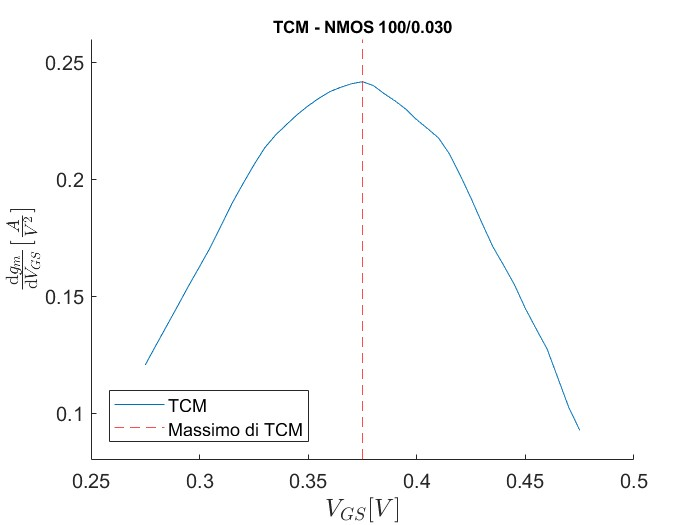
\includegraphics[width=0.49\textwidth]{TCM-N4-100-30-NoFit}
 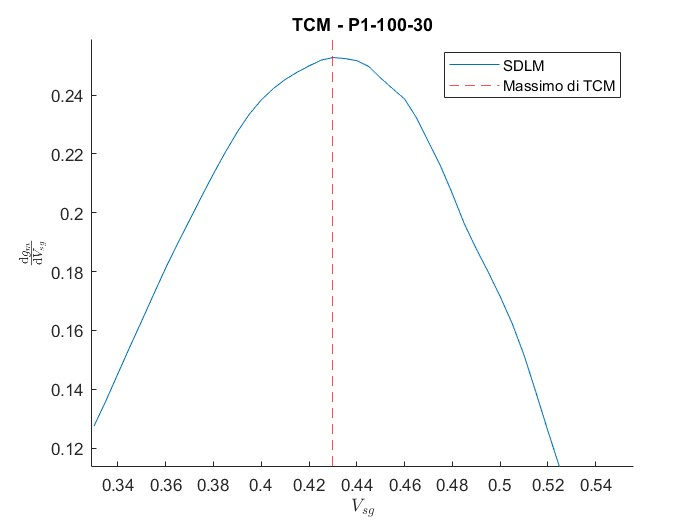
\includegraphics[width=0.49\textwidth]{TCM-P1-100-30-NoFit}
 \caption{Esempio di \emph{TCM} usato su un dispositivo NMOS e un dispositivo PMOS di dimensioni 100-30 a $V_{DS} = 150 mV$}
\end{figure}

Il secondo metodo analizzato è il \emph{Second Difference of the Logarithm of the drain current Minimum method, SDLM}. Questo metodo definisce la $V_{th}$ come la tensione $V_{GS}$ per il quale si ha il picco minimo della derivata seconda del logaritmo naturale di $I_D$ ripetto alla tensione di gate ($\frac{d^2I_D}{dV_{GS}^2}$) ed vale solo per alti valori di $V_{DS}$. \\

\begin{figure}[h!]
\centering
 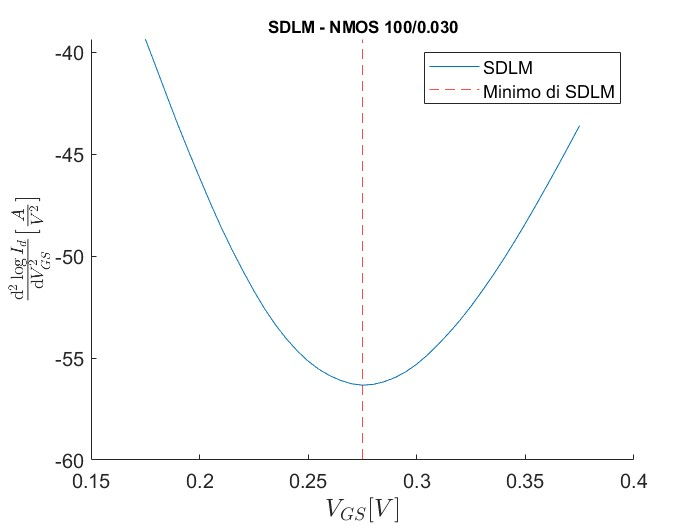
\includegraphics[width=0.49\textwidth]{SDLM-N4-100-30-NoFit}
 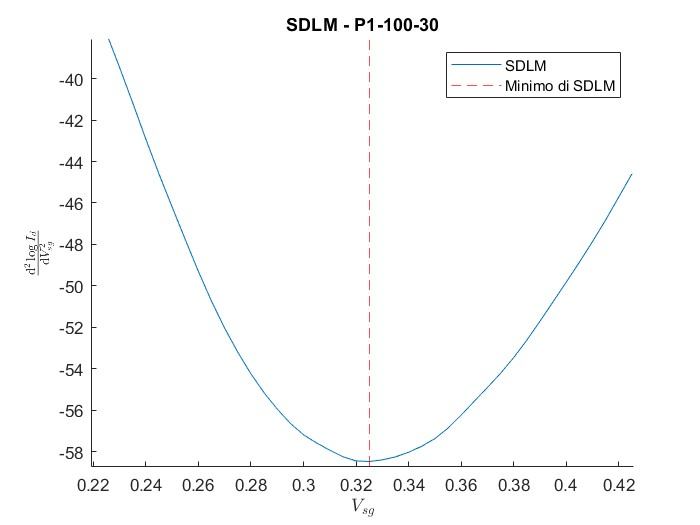
\includegraphics[width=0.49\textwidth]{SDLM-P1-100-30-NoFit}
 \caption{Esempio di \emph{SDLM} usato su un dispositivo NMOS e un dispositivo PMOS di dimensioni 100-30 a $V_{DS} = 900 mV$}
\end{figure}

I due metodi appena esposti, però, sono molto sensibili ai picchi docuti ad errori di misurazione quindi difficilmente utlizzabili, se prima non si rendono i grafici più puliti. Inoltre, la risoluzione del dispositivo di misura utilizzato e di 5 mV, il che rende i valori ottenuti della $V_{th}$ molto approssimativi.
Per far fronte a questi due problemi, si è scelto di non tenere conto del minimo e del massimo direttamente otttenuti dalle derivate delle misurazioni fatte, ma di interpolare prima i punti dei grafici ottenuti con una funzione polinomiale e solo a questo punto di prendere in considerazione i picchi di minimo o di massimo. \\

\begin{figure}[h!]
\centering
 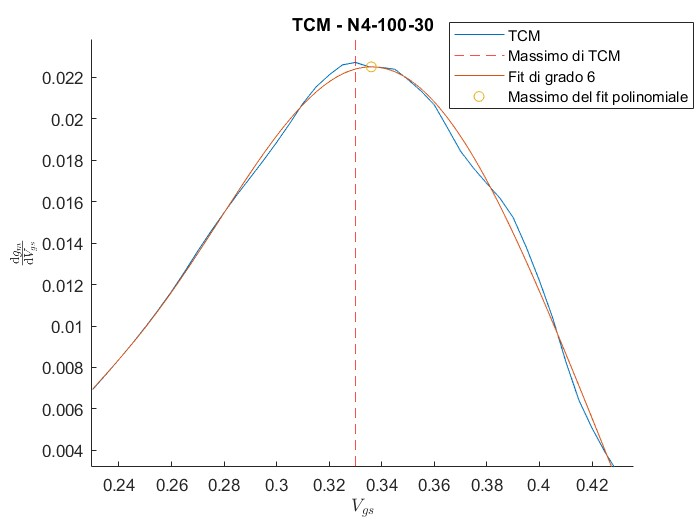
\includegraphics[width=0.49\textwidth]{TCM-N4-100-30}
 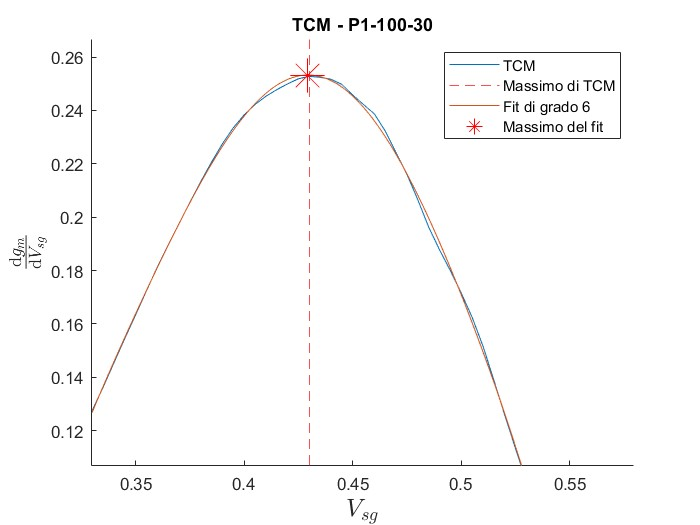
\includegraphics[width=0.49\textwidth]{TCM-P1-100-30}
 \caption{Esempio di \emph{TCM} con fit polinomiale usato su un dispositivo NMOS e un dispositivo PMOS di dimensioni 100-30 a $V_{DS} = 150 mV$}
 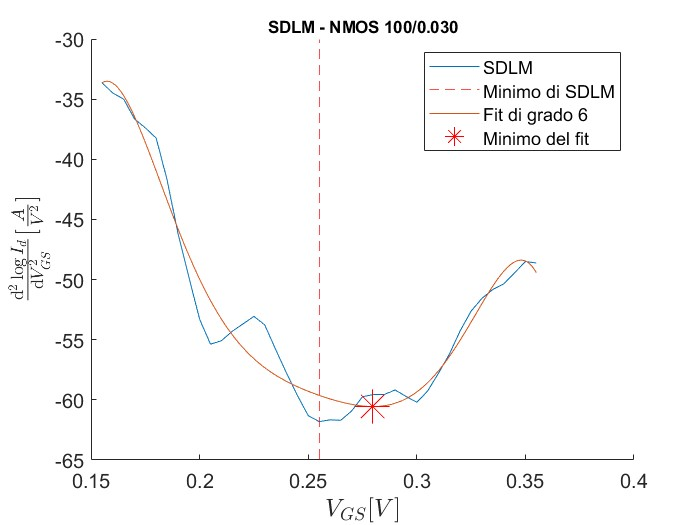
\includegraphics[width=0.49\textwidth]{SDLM-N4-100-30}
 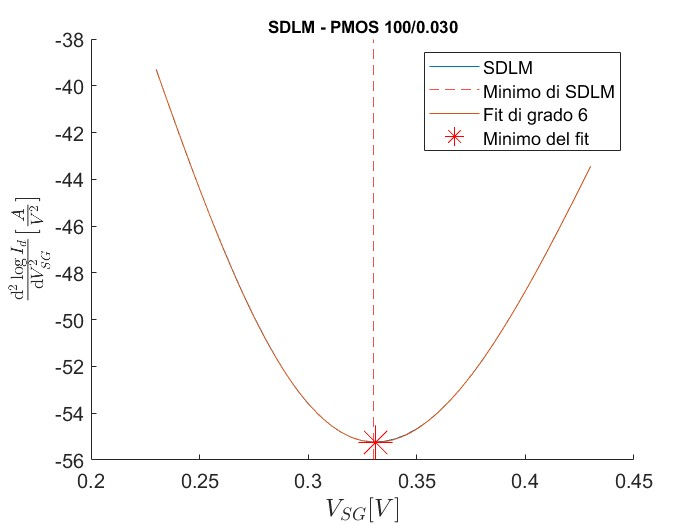
\includegraphics[width=0.49\textwidth]{SDLM-P1-100-30}
 \caption{Esempio di \emph{SDLM} con fit polinomiale usato su un dispositivo NMOS e un dispositivo PMOS di dimensioni 100-30 a $V_{DS} = 900 mV$}
\end{figure}

Per valutare l'accuratezza di questi due metodi si sono quindi calcolate le $V_{th}$ relative ai dispositivi di un PMOS, ottenendo i risultati seguenti:

\begin{center}
\begin{tabular}{c c c}
Dispositivo & TCM ($V_{DS} = 150 mV$) & SDLM ($V_{DS} = 900 mV$) \\
100 - 30  & 0.4806 V & 0.4414 V \\
100 - 60  & 0.4693 V & 0.4116 V \\
200 - 30  & 0.3993 V & 0.2965 V \\
200 - 60  & 0.4535 V & 0.4049 V \\
200 - 180 & 0.4953 V & 0.4493 V \\
600 - 30 & 0.3859 V & 0.2897 V \\
600 - 60 & 0.4347 V & 0.3918 V \\
600 - 180 & 0.4806 V & 0.4414 V \\

\end{tabular}
\end{center}

In generale i risultati sono abbastanza simili tra le due colonne, per cui si potrebbe prendere in considerazione uno di questi due metodi  per estrarre le tensioni di soglia e studiarne la degradazione.\\
È stato però notato un problema non indifferente: il valore della $V_{th}$ estratta dipende dal grado della funzione polinomiale che interpola i punti delle derivate usate per SDLM e TCM. La differenza dei valori estratti al variare del grado non è molto alta, si parla di pochi millivolt, perciò non influenza considerevolmente il valore della singola estrazione. Questa dipendenza, però, è problematica nel momento in cui si vuole studiare con precisione la degradazione della prestazioni di un dispositivo all'aumentare dell'irraggiamento subito, in quanto piccoli spostamenti del valore di $V_{th}$ dovuti alla scelta arbitraria del grado della polinomiale può far variare eccessiavamente le differenze della misurazioni tra un irraggiamento e l'altro, elemento inaccettabile se si considera che già le misure sono influenzate da errori casuali in fase di misurazione.\\\\





Il primo metodo utilizzato è l'\emph{Extrapolation in the Linear Region method, ELR,} con il quale si ottiene la misura della $V_{th}$ attraverso l'analisi della caratteristica $I_D-V_{GS}$. Questo grafico presenta un punto di flesso attorno al quale il grafico è linearizzabile. Tracciando il fit lineare nell'introno del punto di flesso si ottiene un retta che interseca l'asse delle ascisse, ovvero quello di $V_{GS}$ in un punto il cui valore corrisponde a quello della $V_{th}$.\\


\begin{figure}[h!]
\centering
 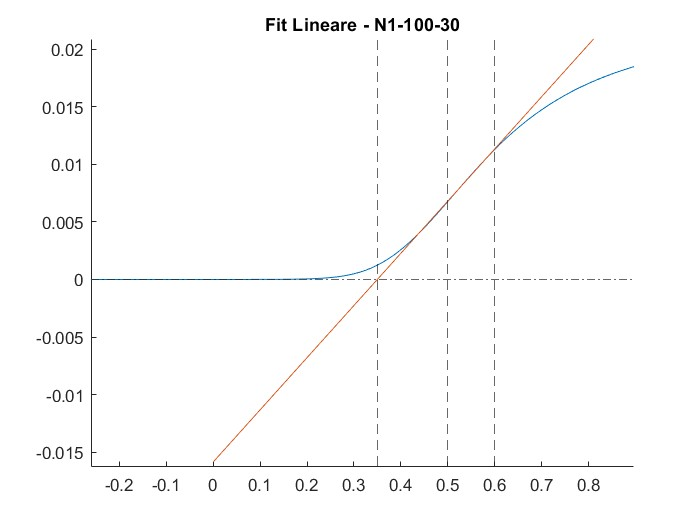
\includegraphics[width=0.49\textwidth]{LinearFit-N1-100-30}
 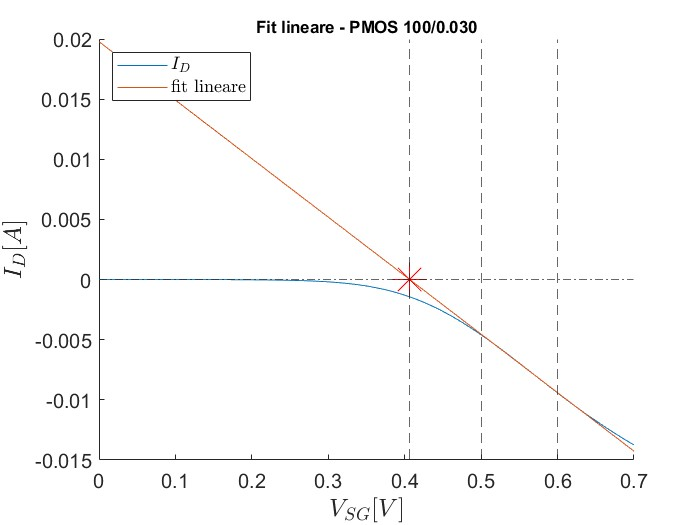
\includegraphics[width=0.49\textwidth]{LinearFit-P1-100-30}
 \caption{Fit lineare della caratteristica  $I_D$-$V_{GS}$ a $V_{DS}=150mV$ di un NMOS e di un PMOS di dimensioni 100-30 nell'intorno $[0,4V ; 0,6V]$ di $V_{GS}$}
\end{figure}














\end{document}